%!TEX root = ../project3.tex
\section{Konzept}
Der Evolutionäre Algorithmus mutiert das Individuum. Im konkreten ist das Individuum ein neuronales Netz. Das Netz wird durch den Algorithmus auf bestimmte Start Konstellationen des Simulators hin trainiert.

Durch verschiedene Anpassungen der Parameter des Algorithmus kann der gesamte Vorgang modifiziert werde um zum Beispiel das Netz zu vergrößern oder Parameter der Mutation anzupassen. Eine Selektion filtert gute und schlechte Individuen welche durch eine Gütefunktion bewertet wurden.

Eine breite Anzahl an Testfällen in unserem Fall verschiedene Simulationsbedingungen ermöglicht das Erzeugen eines möglichst universellen Individuums bzw. Strategie. Dieser Vorgang wird häufig als Training bezeichnet. Das Individuum wird hierbei durch einen Mechanismus auf seine Aufgabe hin optimiert.

\section{Repräsentation}
Die Strategie wird durch ein künstliches neuronales Netz (KNN) entschieden, welches auf bestimmte Eingabewerte hin Entscheidungen trifft und die Verteilung der Aktionspunkte am Simulator vornimmt.

\subsection{Künstliches Neuronale Netz}

Das neuronale Netz besteht im wesentlichen aus einen Eingabeschicht mit neun Neuronen und einer Ausgabeschicht mit sechs Neuronen. Zwischen der ein und Ausgabe sind frei konfigurierbare Layer angeordnet mit gleicher Breite. 

\begin{figure}[h!]
\begin{center}
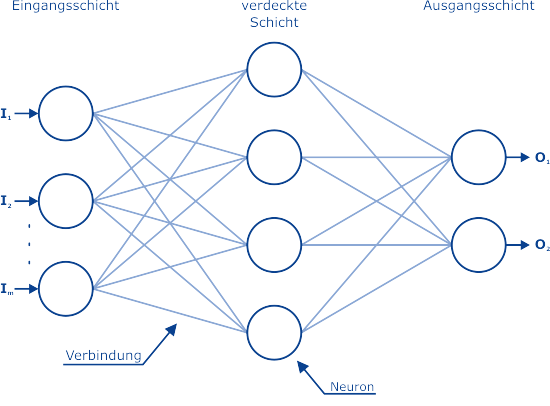
\includegraphics[scale=1.4]{images/knn}
\caption{typischer Aufbau eines KNN;\textit{ Quelle: http://www.lfi.rwth-aachen.de/}}
\label{KNN}
\end{center}
\end{figure}

Die Anzahl ist auch Variabel so kann diese von $1 \cdots n$ festgelegt werden. Diese Schichten werde verdeckte Schicht genannt und sind im Implementierten Individuum voll-vernetzt. Das bedeutet ein Neuron der Schicht \textit{n} gibt seine Informationen an jedes von \textit{n+1} weiter. Schematisch wird dies in (Abb. \ref{KNN}).

\subsection{Neuron}
Das Netz ist eine Sub-Klasse der Individuumsklasse, welche das vorgegebene Interface implementiert. Es beinhaltet eine Liste mit allen Neuronen die im Werte liefern, seinen eigenen Wert, seine Dämpfung wie es Wert aufnimmt und seine Gewichtung wie es seinen Wert weitergibt. Zudem kann ein boolesche Wert gesetzt werden um die Sigmoide Funktion zu verändern.

Es sind 2 Sigmoid-Funktionen implementiert. Funktion \textit{sigmoidOne(x)} berechnet:
\begin{center}$
return = \frac{1}{1+ (-x^{2})}
$\end{center}


und \textit{sigmoidTwo(x}) berechnet:

\begin{center}$
return = \tanh (x)
$\end{center}

\textit{return} bezeichnet den Rückgabewert welche die Java Methode zurückgibt.

\section{Evolutionäre Operatoren}
Ein Neuron des Netzes wird über zwei Parameter gesteuert. Eine Dämpfung ein Gewichtung. Ein Netz aus fünf Schichten jeweils mit fünf Neuronen hat somit $50$ Werte, welche angepasst und mutiert werden müssen. Für die Mutation wird dafür die Selbstadaptive-EP-Mutation verwendet. Diese kann im Detail hier \citep[S.146]{Weicker2007} nachgelesen werden. Eine kurze Beschreibung:

Zu jedem Neuron und dessen zwei Werte existieren zusätzlich zwei Werte welche die Änderungen am Neuron bestimmen. Zunächst verändert die Mutation diese Anpassungsparameter. Nun werden die eigentlichen Werte des Neurons mutiert, hierfür wird der zuvor mutierte Anpassungsparameter einbezogen. Das Ergebnis aus der Mutation sind neue Anpassungsparameter für das Neuron und dessen neuer Gewichtung und Dämpfung.

Der Evolutionsare Operatoren besteht nur aus einer Mutation er hat keine Rekombination.

\section{Selektionsdruck}
Die Population des Evolutionsare Algorithmus ist variable, sie besteht zu beginn aus \textit{x} Eltern Individuen. Diese Werden der Gesamtpopulation hinzugefügt. Die Eltern werden nun mutiert, es entstehen \textit{x} Kind Individuen, welche ebenso der Gesamtpopulation hinzugefügt werden, diese hat nun einen Umfange von \textit{2x} Individuen.

Die Selektion wählt nun die \textit{x} Besten Individuen aus der Population aus welche die neuen Elternindividuen werden. Sie erfolgt über den Gütewert der einzelnen Individuen. Eine Comperator-Methode ermöglicht das sortieren der Listen von Individuen, dadurch wird die Selektion im anschließenden Schritt einfacher.

Ein weitere Selektionsdruck wird nicht angewandt. Ein Archiv welches wären der Laufzeit mit Guten Individuen aufgefüllt ist eine Möglichkeit eine Verbesserung der Selektion zu erzielen. Dabei wir eine kleine Anzahl von guten Individuen gespeichert und eine größere Zahl bei der Selektion verworfen. Leider bliebt dafür nicht genügend Zeit um dieser Möglichkeit in Betracht zu ziehen und weitere Analysen durchzuführen.

\section{Gütebewertung}
Die Gütebewertung der Individuen und deren Strategie wird durch die überlebte Rundenanzahl realisiert. Für gleiche Individuen (überstandene Runden) kann eine weitere Bewertung durch die Bilanz erfolgen. Für das bessere Konditionieren wird ein Individuum mehren Simulationsumgebungen entgegengestellt. Aus dem Durchschnitt aller Einzeltests wird eine Gesamtgüte berechnet welche für die Bewertung bzw. Gegenüberstellung anderer Individuen genutzt wird.

\section{Simulationsszenarien}
Als Ausgangssimulation wurde verwendet \ensuremath{[8, 1, 12, 13, 4, 10, 20, 21, 0]}. Auf Basis dieser wurden $80$ Zufällige Situationen erzeugt, welche sich um ein \ensuremath{\epsilon \approx 3...5}  zum Ursprung unterscheiden können. Ein Paar Beispiele: 
\begin{itemize}
\item\ensuremath{[\overbrace{7}^{Aktionspunkte},\overbrace{1}^{Sanierung},	\overbrace{13}^{Produktion},	\overbrace{12}^{Umweltbelastung},	\overbrace{4}^{Aufklaerung},	11,	20,	21,	1]},
\item\ensuremath{[8,	2,	12,	13,	5,	\overbrace{9}^{Lebensqualitaet}, \overbrace{20}^{Vermehrungsrate},	\overbrace{22}^{Bevoelkerung},	\overbrace{2}^{Politik}]},
\item\ensuremath{[8,	3,	12,	13,	4,	10,	20,	21,	0]},
\item\ensuremath{[7,	2,	11,	12,	3,	9,	19,	20,	1]},
\item\ensuremath{[7,	3,	12,	14,	5,	11,	21,	19,	1]},
\item\ensuremath{[10,	1,	11,	13,	6,	9,	21,	18,	3]}.
\end{itemize}

Anschließend wurde das Individuum gegen eine Auswahl von $5000 - 50000$ Simulationen mit \ensuremath{\epsilon \approx 5} zur Standartvorgabe getestet. Als Ergebnis liefert der Test die durchschnittliche Rundenanzahl sowie Bilanz aller getesteten Vorgaben.

Die als Richtwert vorgegebene Startkonstellation wurde zusätzlich in einem eigenen Test getestet. Das Individuum überlebt $30$ Runden mit einer Bilanz von $8.78\overline{78}$. Speziell auf die Startkonstellation optimierte Individuen liefern eine Bilanz von über $17$. Für extreme Konstellationen liefert das Individuum trotzdem passable Bilanzen und Runden.

Die Testfälle werden durch Zufall erzeugt. Ein Generator bekommt obere und unterer Schranke eines Einzelwertes. Daraufhin werden alle möglichen Belegungen in Array geschrieben. Durch einen Parameter beim Aufruf der Generator Methode kann eine Normalverteilung oder eine Standartverteilung ausgewählt werden. Auf dieser Basis werden anschließend die eigentlichen Werte bestimmt. Ergebnis ist eine zufällig erzeugte Simulator-Startkonstellation. Die beschriebenen Funktionen sind in der Klasse \textit{SimuPipelineGenerator} implementiert.

\section{Effizienz}
Das Individuum besteht aus einem Netz mit acht Layer davon sechs Verdeckte-Layer mit jeweils $16$ Neuronen. Die Laufzeit betrug circa eine halbe Stunde und es mussten fast $2000$ Generationen erzeugt werden. Die insgesamt wurden über $30$ solche Tests gemacht um ein perfektes Individuum zu erzeugen.

Ausschlaggebend für den Erfolg ist jedoch auf welchen Startzustand des Simulators hin optimiert werden soll. Sehr große Startbereiche, Bereiche mit einem großen Epsilon benötigen viel länger und mehr Generationen und erreichen auch nicht die vorgegebene Konditionieren, dass alle Startkonstellationen zu einer maximalen Rundenanzahl von $30$ Runden führen.

Das volle Potential eines Neuronalen Netzes kann erst durch Backtracking-Funktionen ausgeschöpft werden. Diese sind leider explizit untersagt da die Konfiguration des Netzes mit einen evolutionären Algorithmus erzeugt werden \textbf{muss}.

\section{Fazit}
Die Strategie welche im Neuronalen Netz erfasst ist, ist abhängig von der Größe des Netzes. Ein hinreicht großes Netz ist sicher in der Lage für alle Startkonstellationen eine Strategie auszuführen, welche $30$ Runden im Simulator überlebt. Schwachpunkt ist die zu Langsame Mutation die Dauer für die Generierung solch eines Individuums ist enorm.

Hinderlich ist auch der Fakt, durch das Fehler einer Rekombination schnell ein lokales Optima angesteuert wird und das globale mit nur sehr viel Glück erreicht werden kann.

Eine bessere Mutation oder sogar ein Backtracking wären ein Möglichkeit für einen bessere Lösung für die Konfiguration des Individuums. Möglich der Verbesserung wäre verschiedene Berechnungen in Threads zu verlagern und damit die CPU effizienter auszunutzen. Verbesserungspotenzial weist auch die zweite Sigmoide-Funktion auf. Hier kann man durch die Verwendung von vorberechneten Wertetabellen eine Beschleunigung erreichen.

Ein Knackpunkt ist die Implementierung des Pseudozufallszahl-Generator von Java er verbraucht mit Abstand die meiste Laufzeit in der Mutation. Eine effizientere Methode würde die Mutation beschleunigen. Eine alternative ist der Pseudozufallszahl-Generator\footnote{\hyperref[Mersenne-Twister]{http://www.math.sci.hiroshima-u.ac.jp/~m-mat/MT/emt.html}
} von Makoto Matsumoto. Der Generator, welcher zu Testzwecken eingefügt wurde liegt dem Projekt bei er ist unverändert und kann problemlos die \textit{java.util.Random} Methoden ohne viel Aufwand ersetzen.

Eine zusätzliche Testumgebung lädt ein beliebiges Individuum erzeugt eine beliebige Anzahl von Test Simulationen und lässt das Individuum gegen den Simulator antreten. Zehntausend Testfälle werden in weniger als zehn Sekunden abgearbeitet und ausgewertet werden.

Sämtlicher Code liegt dieser Ausarbeitung bei und kann frei verwendet werden. Insgesamt wurde ein vielfaches mehr Zeit für die Bearbeitung und Implementierung des Projektes verwendet als angesetzt wurde.